\documentclass[
11pt, % The default document font size, options: 10pt, 11pt, 12pt
%codirector, % Uncomment to add a codirector to the title page
]{charter} 




% El títulos de la memoria, se usa en la carátula y se puede usar el cualquier lugar del documento con el comando \ttitle
\titulo{Sistema de Iluminación y  Riego por Goteo} 

% Nombre del posgrado, se usa en la carátula y se puede usar el cualquier lugar del documento con el comando \degreename
\posgrado{Carrera de Especialización en Sistemas Embebidos} 
%\posgrado{Carrera de Especialización en Internet de las Cosas} 
%\posgrado{Carrera de Especialización en Intelegencia Artificial}
%\posgrado{Maestría en Sistemas Embebidos} 
%\posgrado{Maestría en Internet de las cosas}

% Tu nombre, se puede usar el cualquier lugar del documento con el comando \authorname
\autor{Ing. Escribá Pedro Santiago} 

% El nombre del director y co-director, se puede usar el cualquier lugar del documento con el comando \supname y \cosupname y \pertesupname y \pertecosupname
\director{Ing. Esp. Brignone Matias Nicolás}
\pertenenciaDirector{Encora} 
% FIXME:NO IMPLEMENTADO EL CODIRECTOR ni su pertenencia
\codirector{John Doe} % para que aparezca en la portada se debe descomentar la opción codirector en el documentclass
\pertenenciaCoDirector{FIUBA}

% Nombre del cliente, quien va a aprobar los resultados del proyecto, se puede usar con el comando \clientename y \empclientename
\cliente{Ing. Rodrigo Fernandez Frittelli}
\empresaCliente{RiegoTec}

% Nombre y pertenencia de los jurados, se pueden usar el cualquier lugar del documento con el comando \jurunoname, \jurdosname y \jurtresname y \perteunoname, \pertedosname y \pertetresname.
\juradoUno{Nombre y Apellido (1)}
\pertenenciaJurUno{pertenencia (1)} 
\juradoDos{Nombre y Apellido (2)}
\pertenenciaJurDos{pertenencia (2)}
\juradoTres{Nombre y Apellido (3)}
\pertenenciaJurTres{pertenencia (3)}
 
\fechaINICIO{20 de octubre de 2022}		%Fecha de inicio de la cursada de GdP \fechaInicioName
\fechaFINALPlan{8 de diciembre de 2022} 	%Fecha de final de cursada de GdP
\fechaFINALTrabajo{16 de octubre de 2023}	%Fecha de defensa pública del trabajo final


\begin{document}

\maketitle
\thispagestyle{empty}
\pagebreak


\thispagestyle{empty}
{\setlength{\parskip}{0pt}
\tableofcontents{}
}
\pagebreak


\section*{Registros de cambios}
\label{sec:registro}


\begin{table}[ht]
\label{tab:registro}
\centering
\begin{tabularx}{\linewidth}{@{}|c|X|c|@{}}
\hline
\rowcolor[HTML]{C0C0C0} 
Revisión & \multicolumn{1}{c|}{\cellcolor[HTML]{C0C0C0}Detalles de los cambios realizados} & Fecha      \\ \hline
0      & Creación del documento                                 &\fechaInicioName \\ \hline
1      & Se completa hasta el punto 5 inclusive                 & 03 de noviembre de 2022 \\ \hline
2      & Se completa hasta el punto 9 inclusive				  & 06 de noviembre de 2022 \\ \hline
%		  Se puede agregar algo más \newline
%		  En distintas líneas \newline
%		  Así                                                    & dd/mm/aaaa \\ \hline
3      & Se completa hasta el punto 12 inclusive                & 12 de noviembre de 2022 \\ \hline
4      & Se completa el plan	                                 & 20 de noviembre de 2022 \\ \hline
\end{tabularx}
\end{table}

\pagebreak



\section*{Acta de constitución del proyecto}
\label{sec:acta}

\begin{flushright}
Buenos Aires, \fechaInicioName
\end{flushright}

\vspace{2cm}

Por medio de la presente se acuerda con el \authorname\hspace{1px} que su Trabajo Final de la \degreename\hspace{1px} se titulará ``\ttitle'', consistirá esencialmente en la implementación de un prototipo de un sistema de riego por goteo, y tendrá un presupuesto preliminar estimado de 600 hs de trabajo y ARS 40700, con fecha de inicio \fechaInicioName\hspace{1px} y fecha de presentación pública \fechaFinalName.

Se adjunta a esta acta la planificación inicial.

\vfill

% Esta parte se construye sola con la información que hayan cargado en el preámbulo del documento y no debe modificarla
\begin{table}[ht]
\centering
\begin{tabular}{ccc}
\begin{tabular}[c]{@{}c@{}}Ariel Lutenberg \\ Director posgrado FIUBA\end{tabular} & \hspace{2cm} & \begin{tabular}[c]{@{}c@{}}\clientename \\ \empclientename \end{tabular} \vspace{2.5cm} \\ 
\multicolumn{3}{c}{\begin{tabular}[c]{@{}c@{}} \supname \\ Director del Trabajo Final\end{tabular}} \vspace{2.5cm} \\
%\begin{tabular}[c]{@{}c@{}}\jurunoname \\ Jurado del Trabajo Final\end{tabular}     &  & \begin{tabular}[c]{@{}c@{}}\jurdosname\\ Jurado del Trabajo Final\end{tabular}  \vspace{2.5cm}  \\
%\multicolumn{3}{c}{\begin{tabular}[c]{@{}c@{}} \jurtresname\\ Jurado del Trabajo Final\end{tabular}} \vspace{.5cm}                                                                     
\end{tabular}
\end{table}




\section{1. Descripción técnica-conceptual del proyecto a realizar}
\label{sec:descripcion}

El objetivo del presente trabajo es implementar nuevas tecnologías a los sistemas de riegos actuales con la finalidad de garantizar un cultivo de excelencia, donde el grado de impacto negativo de las variables climáticas sean lo menor posible. De forma complementaria, se propone también suministrar un sistema de iluminación moderno y vistoso. 

Para cumplimentar con lo recién planteado, se propone utilizar uno o más sensores de humedad por cada cultivo y, mediante un lazo de control cerrado, suministrar el agua que sea requerida. La información para cada especie de planta se encontrará en un servidor virtual y el mismo enviará la información al sistema embebido por Wi-Fi.

A diferencia de otros sistemas de riego, el presente incorpora nuevas tecnologías de comunicación y una interfaz de usuario. Esto permite que cualquier persona con un smarthphone pueda configurar el cultivo asociado a un sensor y obtener estadísticas de la humedad de la tierra así como controlar un arreglo de LEDs RGB situado cercano a un sensor o plantín.

En la Figura \ref{fig:diagBloques} se puede observar los diferentes bloques del proyecto, seccionado de acuerdo a las tecnologías a utilizar. La interfaz de usuario abarca el alto nivel tecnológico y más cercano a la persona, mientras que el sistema embebido representa el bajo nivel tecnológico y más lejano a la persona.

\begin{figure}[htpb]
\centering 
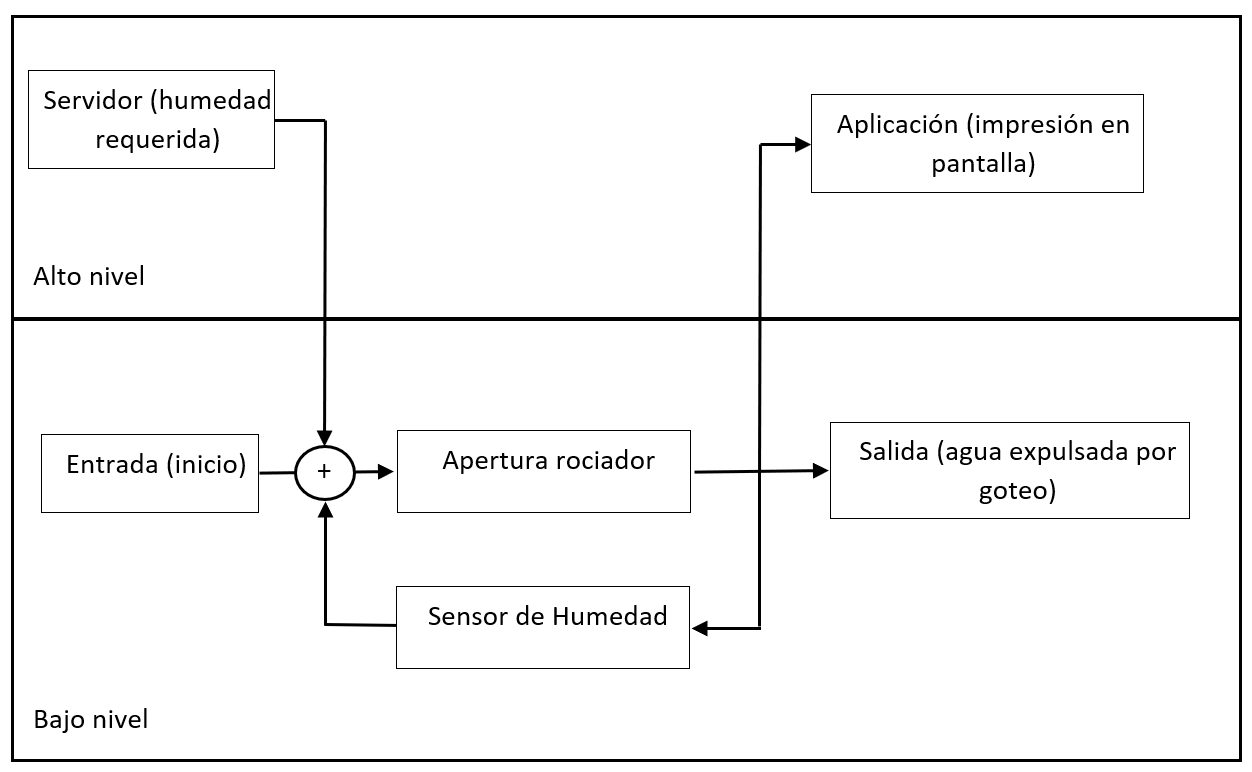
\includegraphics[width=1\textwidth]{./Figuras/digBloq.png}
\caption{Diagrama en bloques del sistema.}
\label{fig:diagBloques}
\end{figure}


\section{2. Identificación y análisis de los interesados}
\label{sec:interesados}

En esta sección se presentan los interesados en el proyecto. En la Tabla \ref{tab:interesados} se puede apreciar los distintos roles, organización y puesto de las personas que poseen un cierto interés en el producto a desarrollar.

\begin{table}[ht]
%\caption{Identificación de los interesados}
%\label{tab:interesados}
\begin{tabularx}{\linewidth}{@{}|l|X|X|l|@{}}
\hline
\rowcolor[HTML]{C0C0C0} 
Rol           & Nombre y Apellido & Organización 	& Puesto 	\\ \hline
Auspiciante   & \clientename      &\empclientename 	& -        	\\ \hline
Cliente       & \clientename      &\empclientename	& -      	\\ \hline
Responsable   & \authorname       & FIUBA        	& Alumno 	\\ \hline
Orientador    & \supname	      & \pertesupname 	& Director Trabajo final \\ \hline
Usuario final & Ana Fernandez     &Particular    	& -       	\\ \hline
\end{tabularx}
\caption{Interesados}
\label{tab:interesados}
\end{table}

\begin{itemize}
	\item Auspiciante y Cliente: es riguroso y exigente. Desea un producto final en condiciones óptimas y sin fallas.
	\item Orientador: Matías es un profesional de excelencia, capaz de asistir en las necesidades que surjan.
	\item Usuario final: profesional de herbología.
\end{itemize}



\section{3. Propósito del proyecto}
\label{sec:proposito}

El propósito de este proyecto es diseñar un prototipo funcional capaz de administrar agua mediante la tecnología de goteo a un cultivo determinado, satisfaciendo las necesidades del cliente involucrado. A su vez, se pretende aplicar los conocimientos adquiridos en la carrera de especialización de Sistemas Embebidos permitiendo que los mismos sean afianzados.


\section{4. Alcance del proyecto}
\label{sec:alcance}

Acorde a las necesidades del cliente, el proyecto incluye el desarrollo de un firmware en lenguaje C encargado del control a lazo cerrado del sistema de riego y su comunicación con un servidor. También es parte de este proyecto el desarrollo mecánico de un prototipo funcional de riego por goteo que responda a las necesidades de un único cultivo. Además, se incluye el código para el control del sistema de iluminación y su desarrollo físico y, por último, una demo de una interfaz de usuario para utilizar en smartphones.

En cambio, no es parte de este proyecto el desarrollo del código de la interfaz de usuario y brindar soporte a la misma. Tampoco se incluye el desarrollo de un PBC para alojar los diferentes componentes ni el desarrollo del hardware necesario.


\section{5. Supuestos del proyecto}
\label{sec:supuestos}

Para el desarrollo del presente proyecto se supone que:

\begin{itemize}
	\item Se conocen todos los conceptos técnicos necesarios para su desarrollo. 
	\item Se dispone de los recursos económicos como de los materiales.
	\item Se dispone de un tiempo acotado a las necesidades del cliente: el proyecto se debe ejecutar en dos meses.
	\item El director del proyecto tendrá su participación, brindando ideas y corrigiendo errores.
	\item El impacto de las condiciones macroeconómicas y reglamentarias será mínimo.
\end{itemize}

\section{6. Requerimientos}
\label{sec:requerimientos}

En la siguiente sección se enumeran los requerimientos del proyecto propuesto.
\begin{enumerate}
	\item Requerimientos funcionales del firmware:
		\begin{enumerate}
			\item Debe estar codificado en lenguaje C.
			\item Debe incluir un sistema operativo de tiempo real.
			\item Debe ser portable a otras plataformas.
			\item Debe ser escalable a múltiples goteros.
			\item El código debe ser prolijo, legible y entendible.
%			\item Debe aplicar los conocimientos adquiridos a lo largo de la cursada de la especialidad en Sistemas Embebidos.
		\end{enumerate}
	\item Requerimientos funcionales de hardware:
		\begin{enumerate}
			\item Deben utilizarse el módulo ESP32 de Espressif como controlador general.
			\item Deben utilizarse las placas de evaluación sin la necesidad de realizar un PCB.
			\item Los sensores de humedad deben ser del modelo HD38.
			\item Se debe garantizar la tensión y corriente mínima para alimentar el sistema de iluminación y el mecanismo de goteo de acuerdo a especificaciones de las hojas de datos.
			\item Toda la electrónica sin uso directo (es decir aquello que no sean sensores, luces o cableado) debe estar bajo una protección de humedad IP23.
%			\item Debe aplicar los conocimientos adquiridos a lo largo de la cursada de la especialidad en Sistemas Embebidos.
		\end{enumerate}
	\item Requerimientos funcionales de la Interfaz de Usuario:
		\begin{enumerate}
			\item Deben ser apta para smartphone.
			\item Deben tener diseño responsivo.
		\end{enumerate}
	\item Requerimientos de documentación
		\begin{enumerate}
			\item La documentación debe presentarse en formato PDF usando lenguaje Latex.
			\item Debe presentarse un manual de usuario que explique el funcionamiento del producto.
		\end{enumerate}
\end{enumerate}

\section{7. Historias de usuarios (\textit{Product backlog})}
\label{sec:backlog}

A continuación se adjuntan las principales Historias de usuarios. Para valorarlas se propone un sistema de puntos continuos entre 0 y 10, ponderando la dificultad, la complejidad y la incertidumbre (o riesgo involucrado) del requerimiento planteado en la historia. De esta forma, para comparar entre historias, se calcula el esfuerzo requerido a partir de la suma de los puntos y estimado de acuerdo a la serie de Fibonacci, aproximando al valor más cercano.
\begin{enumerate}
	\item ''Como usuario quiero un sistema de riego para no perder tiempo regando plantas''.
	\begin{enumerate}
		\item Dificultad: 8 puntos.
		\item Complejidad: 5 puntos.
		\item Incertidumbre: 7 puntos.
		\item Total: 20 puntos, Fibonacci más cercano 21.
	\end{enumerate}
	\item ''Como herbóloga deseo que mis plantas tengan la humedad correcta para tener un cultivo de excelencia''.
	\begin{enumerate}
		\item Dificultad: 5 puntos.
		\item Complejidad: 8 puntos.
		\item Incertidumbre: 4 puntos.
		\item Total: 17 puntos, Fibonacci más cercano 21.
	\end{enumerate}
	\item ''Como expositor de cultivos quiero una iluminación precisa para ganar valor cultural''.
	\begin{enumerate}
		\item Dificultad: 3 puntos.
		\item Complejidad: 4 puntos.
		\item Incertidumbre: 1 puntos.
		\item Total: 8 puntos, Fibonacci más cercano 8.
	\end{enumerate}
	\item ''Como herbóloga quiero disponer de toda la información del riego en mi celular para un mejor control''.
	\begin{enumerate}
		\item Dificultad: 5 puntos.
		\item Complejidad: 2 puntos.
		\item Incertidumbre: 0 puntos.
		\item Total: 7 puntos, Fibonacci más cercano 7.
	\end{enumerate}
\end{enumerate}

\section{8. Entregables principales del proyecto}
\label{sec:entregables}

A continuación se enumeran los entregables que dispondrá este proyecto:
\begin{itemize}
	\item Hardware funcional basado en módulo ESP32.
	\item Manual de usuario.
	\item Guía de instalación.
	\item Diagrama de circuitos esquemáticos.
	\item Hoja de datos de los dispositivos involucrados.
	\item Código fuente del firmware.
	\item Informe final.

\end{itemize}

\section{9. Desglose del trabajo en tareas}
\label{sec:wbs}

De acuerdo a los requerimientos planteados en la sección \ref{sec:requerimientos} se proyecta el siguiente desglose de tareas.
\begin{enumerate}
\item Firmware y software.
	\begin{enumerate}
	\item Investigación de productos existentes y necesidades del cliente (30 hs).
	\item Planificación del diseño (30 hs).
	\item Planificación del proyecto (40 hs).
	\item Planificación y diseño del firmware (13 hs).
	\item Desarrollo del código fuente de la Maquina de Estados (30 hs).
	\item Desarrollo del código fuente del Sistema Operativo en Tiempo Real (35 hs).
	\item Desarrollo de servidor web (30 hs).
	\item Desarrollo de aplicación de usuario (30 hs).
	\end{enumerate}
\item Hardware.
	\begin{enumerate}
	\item Planificación y diseño del hardware(12 hs).
	\item Adquisición de insumos (10 hs).
	\item Armado del prototipo de riego (35 hs).
	\item Armado del prototipo de iluminación (25 hs).
	\end{enumerate}
\item Testing.
	\begin{enumerate}
	\item Pruebas del hardware (40 hs).
	\item Pruebas del firmware (40 hs).
	\end{enumerate}
\item Documentación.
	\begin{enumerate}
	\item Documentación del código fuente (30 hs).
	\item Documentación del diseño (30 hs).
	\item Armado de documentación, guía de usuario y diagramado (40 hs).
	\item Desarrollo del informe de avance (30 hs).
	\item Desarrollo de la memoria técnica (70 hs).
	\end{enumerate}
\end{enumerate}

Cantidad total de horas: (600 hs).

\section{10. Diagrama de Activity On Node}
\label{sec:AoN}

A partir del desglose de tareas de la sección \ref{sec:wbs}, se genera el diagrama de Activity On Node de la figura \ref{fig:AoN}.

\begin{figure}[htpb]
\centering 
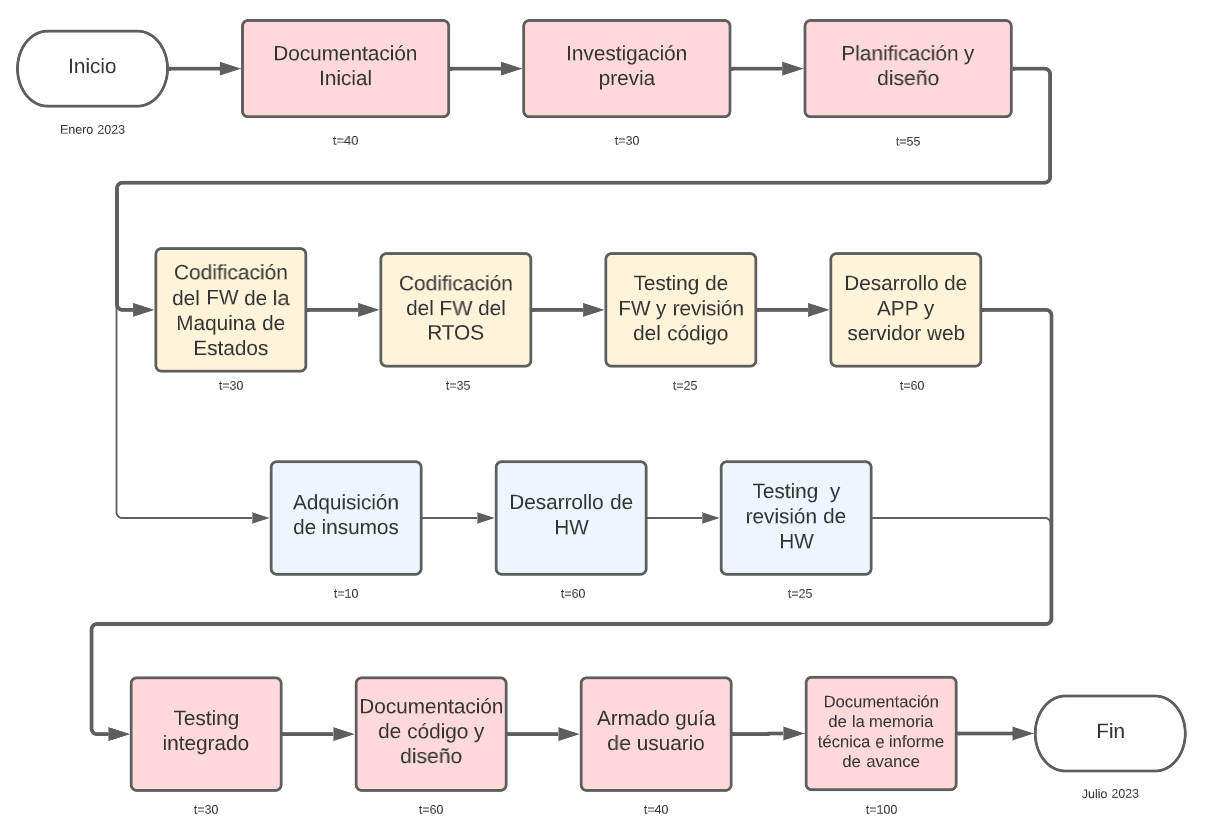
\includegraphics[width=1\textwidth]{./Figuras/diagAoN.png}
\caption{Activity on Node. El color rojo representa las tareas de documentación, el color amarillo las tareas relativas al firmware y el azul las relativas al hardware. La unidad de tiempo es la hora.}
\label{fig:AoN}
\end{figure}

\section{11. Diagrama de Gantt}
\label{sec:gantt}

En la figura \ref{fig:diagGantt} se presenta un diagrama de Gantt con la planificación de las tareas analizadas en la sección \ref{sec:wbs}. En este caso se analiza cómo se distribuirán las tareas a lo largo de los diferentes meses de trabajo, partiendo de que el inicio de las actividades será en el mes de Enero del 2023 y finalizará en Septiembre de 2023. Para este diagrama se calculan entre 10 y 15 horas de trabajo por semana aproximadamente, cantidad que puede variar de acuerdo a la demanda de trabajo. A su vez en la tabla \ref{tab:tabGantt} se observa en detalle las fechas de inicio y finalización de cada tarea, así como su duración y predecesora.

\begin{table}[htpb]
\centering
\begin{tabularx}{\linewidth}{@{}|c|X|X|c|c|c|c|@{}}
\hline
\rowcolor[HTML]{C0C0C0} 
Gantt ID & Tareas ID & Nombre de la Tarea & Duración & Comienzo & Fin & Predecesora \\ \hline
1&1.1&Documentación Preliminar.&40 hs&02/01/2023&21/02/2023&-\\ \hline
2&1.2, 1.3, 1.4 y 2.1&Investigación y Planificación.&85 hs&22/01/2023&28/02/2023&1\\ \hline
3&2.2&Adquisición de insumos.&10 hs&08/02/2023&21/02/2023&2\\ \hline
4&1.5&Desarrollo FW Maquina de Estados.&30 hs&01/03/2023&07/04/2023&2\\ \hline
5&1.6&Desarollo FW RTOS.&35 hs&01/03/2023&14/04/2023&2\\ \hline
6&3.2&Testing FW.&40 hs&01/04/2023&30/04/2023&4, 5\\ \hline
7&2.3 y 2.4&Desarrollo HW.&60 hs&15/04/2023&31/05/2023&2, 3, 6\\ \hline
8&3.1&Testing HW.&40 hs&15/05/2023&21/06/2023&7\\ \hline
9&1.7 y 1.8&Desarrollo APP.&60 hs&22/06/2023&14/07/2023&2, 6\\ \hline
10&4.1, 4.2 y 4.3&Documentación de código y diseño.&60 hs&15/07/2023&07/08/2023&2, 9\\ \hline
11&4.4 y 4.5&Desarrollo de Memoria Técnica y Presentación.&140 hs&15/07/2023&30/09/2023&2, 9\\ \hline
\end{tabularx}%
\caption{Tareas de gantt.}
\label{tab:tabGantt}
\end{table}

\begin{landscape}
\begin{figure}[htpb]
\centering 
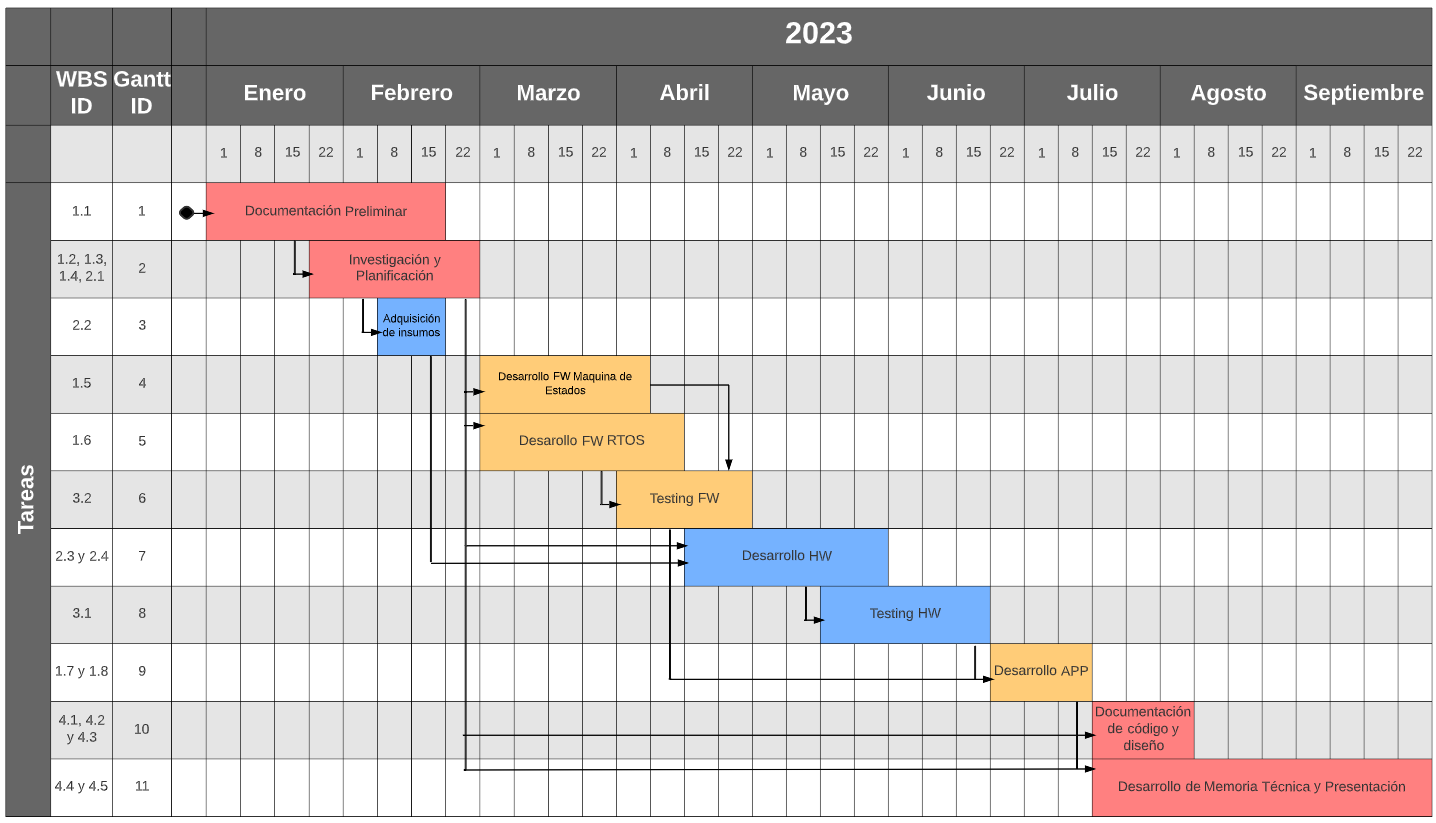
\includegraphics[height=.85\textheight]{./Figuras/diagGantt.png}
\caption{Diagrama de Gantt. El color rojo representa las tareas de documentación, el color amarillo las tareas relativas al firmware y el azul las relativas al hardware.}
\label{fig:diagGantt}
\end{figure}

\end{landscape}


\section{12. Presupuesto detallado del proyecto}
\label{sec:presupuesto}

Esta sección presenta un presupuesto detallado requerido para el desarrollo del proyecto. En la tabla \ref{tab:presupuesto} se encuentran los costos tanto directos como indirectos, subtotales y totales.

\begin{table}[htpb]
\centering
\begin{tabularx}{\linewidth}{@{}|X|c|r|r|@{}}
\hline
\rowcolor[HTML]{C0C0C0} 
\multicolumn{4}{|c|}{\cellcolor[HTML]{C0C0C0}COSTOS DIRECTOS} \\ \hline
\rowcolor[HTML]{C0C0C0} 
Descripción &
  \multicolumn{1}{c|}{\cellcolor[HTML]{C0C0C0}Cantidad} &
  \multicolumn{1}{c|}{\cellcolor[HTML]{C0C0C0}Valor unitario} &
  \multicolumn{1}{c|}{\cellcolor[HTML]{C0C0C0}Valor total} \\ \hline
 Módulo ESP32&
  \multicolumn{1}{c|}{1} &
  \multicolumn{1}{c|}{800} &
  \multicolumn{1}{c|}{800} \\ \hline
 Sensor HD38&
  \multicolumn{1}{c|}{3} &
  \multicolumn{1}{c|}{3500} &
  \multicolumn{1}{c|}{10500} \\ \hline
 Manguera de riego polietireno 1/2''&
  \multicolumn{1}{c|}{2} &
  \multicolumn{1}{c|}{250} &
  \multicolumn{1}{c|}{500} \\ \hline
 Gotero&
  \multicolumn{1}{c|}{3} &
  \multicolumn{1}{c|}{500} &
  \multicolumn{1}{c|}{1500} \\ \hline
 Bomba para control de gotero&
  \multicolumn{1}{c|}{3} &
  \multicolumn{1}{c|}{3500} &
  \multicolumn{1}{c|}{10500} \\ \hline
 Pack Cables Macho-Hembra&
  \multicolumn{1}{c|}{2} &
  \multicolumn{1}{c|}{700} &
  \multicolumn{1}{c|}{1400} \\ \hline
 Caja protección IP23&
  \multicolumn{1}{c|}{1} &
  \multicolumn{1}{c|}{1500} &
  \multicolumn{1}{c|}{1500} \\ \hline
\multicolumn{3}{|c|}{SUBTOTAL} &
  \multicolumn{1}{c|}{26700} \\ \hline
\rowcolor[HTML]{C0C0C0} 
\multicolumn{4}{|c|}{\cellcolor[HTML]{C0C0C0}COSTOS INDIRECTOS} \\ \hline
\rowcolor[HTML]{C0C0C0} 
Descripción &
  \multicolumn{1}{c|}{\cellcolor[HTML]{C0C0C0}Cantidad} &
  \multicolumn{1}{c|}{\cellcolor[HTML]{C0C0C0}Valor unitario} &
  \multicolumn{1}{c|}{\cellcolor[HTML]{C0C0C0}Valor total} \\ \hline
 Electricidad&
  \multicolumn{1}{c|}{6 meses} &
  \multicolumn{1}{c|}{1000} &
  \multicolumn{1}{c|}{6000} \\ \hline
 Internet&
  \multicolumn{1}{c|}{6 meses} &
  \multicolumn{1}{c|}{2000} &
  \multicolumn{1}{c|}{12000} \\ \hline
\multicolumn{3}{|c|}{SUBTOTAL} &
  \multicolumn{1}{c|}{14000} \\ \hline
\rowcolor[HTML]{C0C0C0}
\multicolumn{3}{|c|}{TOTAL} & 40700
   \\ \hline
\end{tabularx}%
\caption{Presupuesto del proyecto expresado en ARS.}
\label{tab:presupuesto}
\end{table}


\section{13. Gestión de riesgos}
\label{sec:riesgos}

En esta sección se identifican los principales riesgos del proyecto y sus consecuencias, así como el plan de mitigación para cada caso.

Riesgo 1: imposibilidad de responder de acuerdo a los tiempos planteado en la sección \ref{sec:gantt}.
\begin{itemize}
	\item Severidad (S): 8, dado que deberán replantearse los tiempos de desarrollo y no cumplir con la meta final.
	\item Probabilidad de ocurrencia (O): 7, dado que hay nuevos desafíos laborales planteado que demandaran mayor tiempo de trabajo. 
\end{itemize}

Riesgo 2: no conseguir los componentes necesarios.
\begin{itemize}
	\item Severidad (S): 8, ya que no podrá construirse el prototipo de testeo.
	\item Probabilidad de ocurrencia (O): 3, ya que son componentes de fácil acceso y de fabricación nacional. 
\end{itemize}

Riesgo 3: incurrir en gastos mayores a los presupuestados.
\begin{itemize}
	\item Severidad (S): 3, dado que se deberá gastar mayor cantidad de dinero.
	\item Probabilidad de ocurrencia (O): 9, dado el contexto inflacionario del país. 
\end{itemize}

Riesgo 4: no disponer de los conocimientos técnicos a tiempo.
\begin{itemize}
	\item Severidad (S): 7, ya que imposibilitará continuar con un proyecto de calidad.
	\item Probabilidad de ocurrencia (O): 7, ya que se iniciará el proyecto en simultaneo a la cursada de la carrera. 
\end{itemize}

Riesgo 5: cancelación del proyecto por parte del cliente.
\begin{itemize}
	\item Severidad (S): 9, dado que el proyecto no se podrá realizar.
	\item Probabilidad de ocurrencia (O): 2, dado el alto interés del cliente en el producto. 
\end{itemize}

La tabla \ref{tab:riesgos} muestra la matriz de gestión de riesgos, donde RPN se calcula como SxO.
\begin{table}[htpb]
\centering
\begin{tabularx}{\linewidth}{@{}|X|c|c|c|c|c|c|@{}}
\hline
\rowcolor[HTML]{C0C0C0} 
Riesgo & S & O & RPN & S* & O* & RPN* \\ \hline
Imposibilidad de responder de acuerdo a los tiempos planteado en el Diagrama de Gantt.&8&7&56&5&2&10\\ \hline
No conseguir los componentes necesarios.&8&3&24&-&-&-\\ \hline
Incurrir en gastos mayores a los presupuestados.&3&9&18&-&-&-\\ \hline
No disponer de los conocimientos técnicos a tiempo.&7&7&49&2&1&2\\ \hline
Cancelación del proyecto por parte del ciente.&9&2&18&-&-&-\\ \hline
\end{tabularx}%
\caption{Gestión de riesgos.}
\label{tab:riesgos}
\end{table}

A continuación se establece el plan de mitigación de los riesgos cuyo RPN es mayor a 25 puntos.

Riesgo 1: imposibilidad de responder de acuerdo a los tiempos planteado en la sección \ref{sec:gantt}. Se mitigará adaptando el cronograma de trabajo teniendo en cuenta las dificultades que surjan en el camino. También se hablará con el cliente para coordinar nuevos tiempos de entrega.
\begin{itemize}
	\item Severidad (S): 5, dado que habrá un nuevo tiempo de entrega.
	\item Probabilidad de ocurrencia (O): 2, ya que se tendrá más información de avances y la realimentación de tiempos será más exacta. 
\end{itemize}

Riesgo 4: no disponer de los conocimientos técnicos a tiempo. Se mitigará adquiriendo los conocimientos necesarios de manera extracurricular.
\begin{itemize}
	\item Severidad (S): 2, dado que se dispone de los materiales de estudio.
	\item Probabilidad de ocurrencia (O): 1, ya que los conocimientos serán adquiridos correctamente. 
\end{itemize}


\section{14. Gestión de la calidad}
\label{sec:calidad}
La gestión de la calidad es una parte importante del proyecto, es por ello que se realiza el análisis para cada uno de los requerimientos mencionados en la sección \ref{sec:requerimientos}.

\begin{itemize} 
\item Req \#1: Debe estar codificado en lenguaje C.
\begin{itemize}
	\item Verificación: se leerá el código fuente.
	\item Validación: el mismo debe compilar con un IDE configurado en lenguaje C.
\end{itemize}

\item Req \#2: Debe ser portable a otras plataformas.
\begin{itemize}
	\item Verificación: se compilará para otras plataformas.
	\item Validación: se mostrará al cliente el mismo código corriendo en otra plataforma.
\end{itemize}

\item Req \#3: Debe ser escalable a múltiples goteros.
\begin{itemize}
	\item Verificación: se realizarán simulaciones con múltiples goteros.
	\item Validación: se mostrará al cliente dichas simulaciones.
\end{itemize}

\item Req \#4: El código debe ser prolijo, legible y entendible.
\begin{itemize}
	\item Verificación: se leerá el código y debe ser entendido por un programador ajeno al proyecto.
	\item Validación: el código formará parte de la documentación.
\end{itemize}

\item Req \#5: Deben utilizarse el módulo ESP32 de Espressif como controlador general.
\begin{itemize}
	\item Verificación: se dispondrá del módulo especificado.
	\item Validación: se realizarán pruebas de funcionamiento en dicho módulo.
\end{itemize}

\item Req \#6: Deben utilizarse las placas de evaluación sin la necesidad de realizar un PCB.
\begin{itemize}
	\item Verificación: se dispondrá de las placas de evaluación especificadas.
	\item Validación: se realizarán pruebas de funcionamiento en dichas placas.
\end{itemize}

\item Req \#7: Los sensores de humedad deben ser del modelo HD38.
\begin{itemize}
	\item Verificación: se dispondrá de los módulos especificados.
	\item Validación: se realizarán pruebas de funcionamiento en dichos módulos.
\end{itemize}

\item Req \#8: Se debe garantizar la tensión y corriente mínima para alimentar el sistema de iluminación y el mecanismo de goteo de acuerdo a especificaciones de las hojas de datos.
\begin{itemize}
	\item Verificación: se realizarán cálculos de tensión y corriente de acuerdo a las especificaciones técnicas.
	\item Validación: se medirá tensión y corriente en todo el sistema.
\end{itemize}

\item Req \#9: Toda la electrónica sin uso directo (es decir aquello que no sean sensores, luces o cableado) debe estar bajo una protección de humedad IP23.
\begin{itemize}
	\item Verificación: se revisará los productos seleccionados para que cumplan con dicho requerimiento.
	\item Validación: se realizarán pruebas de humedad para validar la calidad del prototipo.
\end{itemize}

\item Req \#10: Aplicación de usuario debe ser apta para smartphone.
\begin{itemize}
	\item Verificación: se diseñará con programas cuyas especificaciones permitan el uso en smartphones.
	\item Validación: se correrá en un smartphone con sistema operativo Android.
\end{itemize}

\item Req \#11: Deben tener diseño responsivo.
\begin{itemize}
	\item Verificación: se realizará una prueba de uso por un usuario con conocimientos.
	\item Validación: se realizará una prueba de uso por un usuario sin conocimientos.
\end{itemize}

\item Req \#12: La documentación debe presentarse en formato PDF usando lenguaje Latex.
\begin{itemize}
	\item Verificación: se leerá el código fuente.
	\item Validación: la misma debe ser leída en un lector PDF y disponer del formato correspondiente a la plantilla planteada.
\end{itemize}

\item Req \#13: Debe presentarse un manual de usuario que explique el funcionamiento del producto
\begin{itemize}
	\item Verificación: se leerá el manual de usuario.
	\item Validación: dicho manual será leído por un usuario sin conocimientos.
\end{itemize}
\end{itemize}


\section{15. Procesos de cierre}    
\label{sec:cierre}

Finalmente, se analizan las pautas de trabajo para realizar una reunión final de evaluación del proyecto, las cuales contemplan las siguientes actividades:

\begin{itemize}
	\item Pautas de trabajo que se seguirán para analizar si se respetó el Plan de Proyecto original:
	 - El estudiante y el director se reunirán para analizar si se respetó el Plan de Proyecto original. En dicha reunión se dispondrá de este documento y se estudiará punto a punto que cada objetivo planteado haya sido cumplido. También se analizarán los riesgos asumidos y el correcto cumplimiento de los requisitos planteados.
	 
	\item Identificación de las técnicas y procedimientos útiles e inútiles que se emplearon, y los problemas que surgieron y cómo se solucionaron:
	 - El estudiante hará un análisis de cada procedimiento que empleó y dejará constancia en un documento de los pros y contras de cada técnica utilizada, así como de los problemas que surgieron y las soluciones empleadas.
	 
	\item Indicar quién organizará el acto de agradecimiento a todos los interesados, y en especial al equipo de trabajo y colaboradores:
	  - El estudiante será el encargado de dicha tarea y la misma se llevará a cabo el día de la presentación del trabajo final.
\end{itemize}

\end{document}
